\begin{frame}{ASM, RAS Smoothers}
  \begin{figure} \centering
  {\setlength{\unitlength}{1\textwidth}
    \begin{picture}(1,0.35)
       \put(0.0,0.0){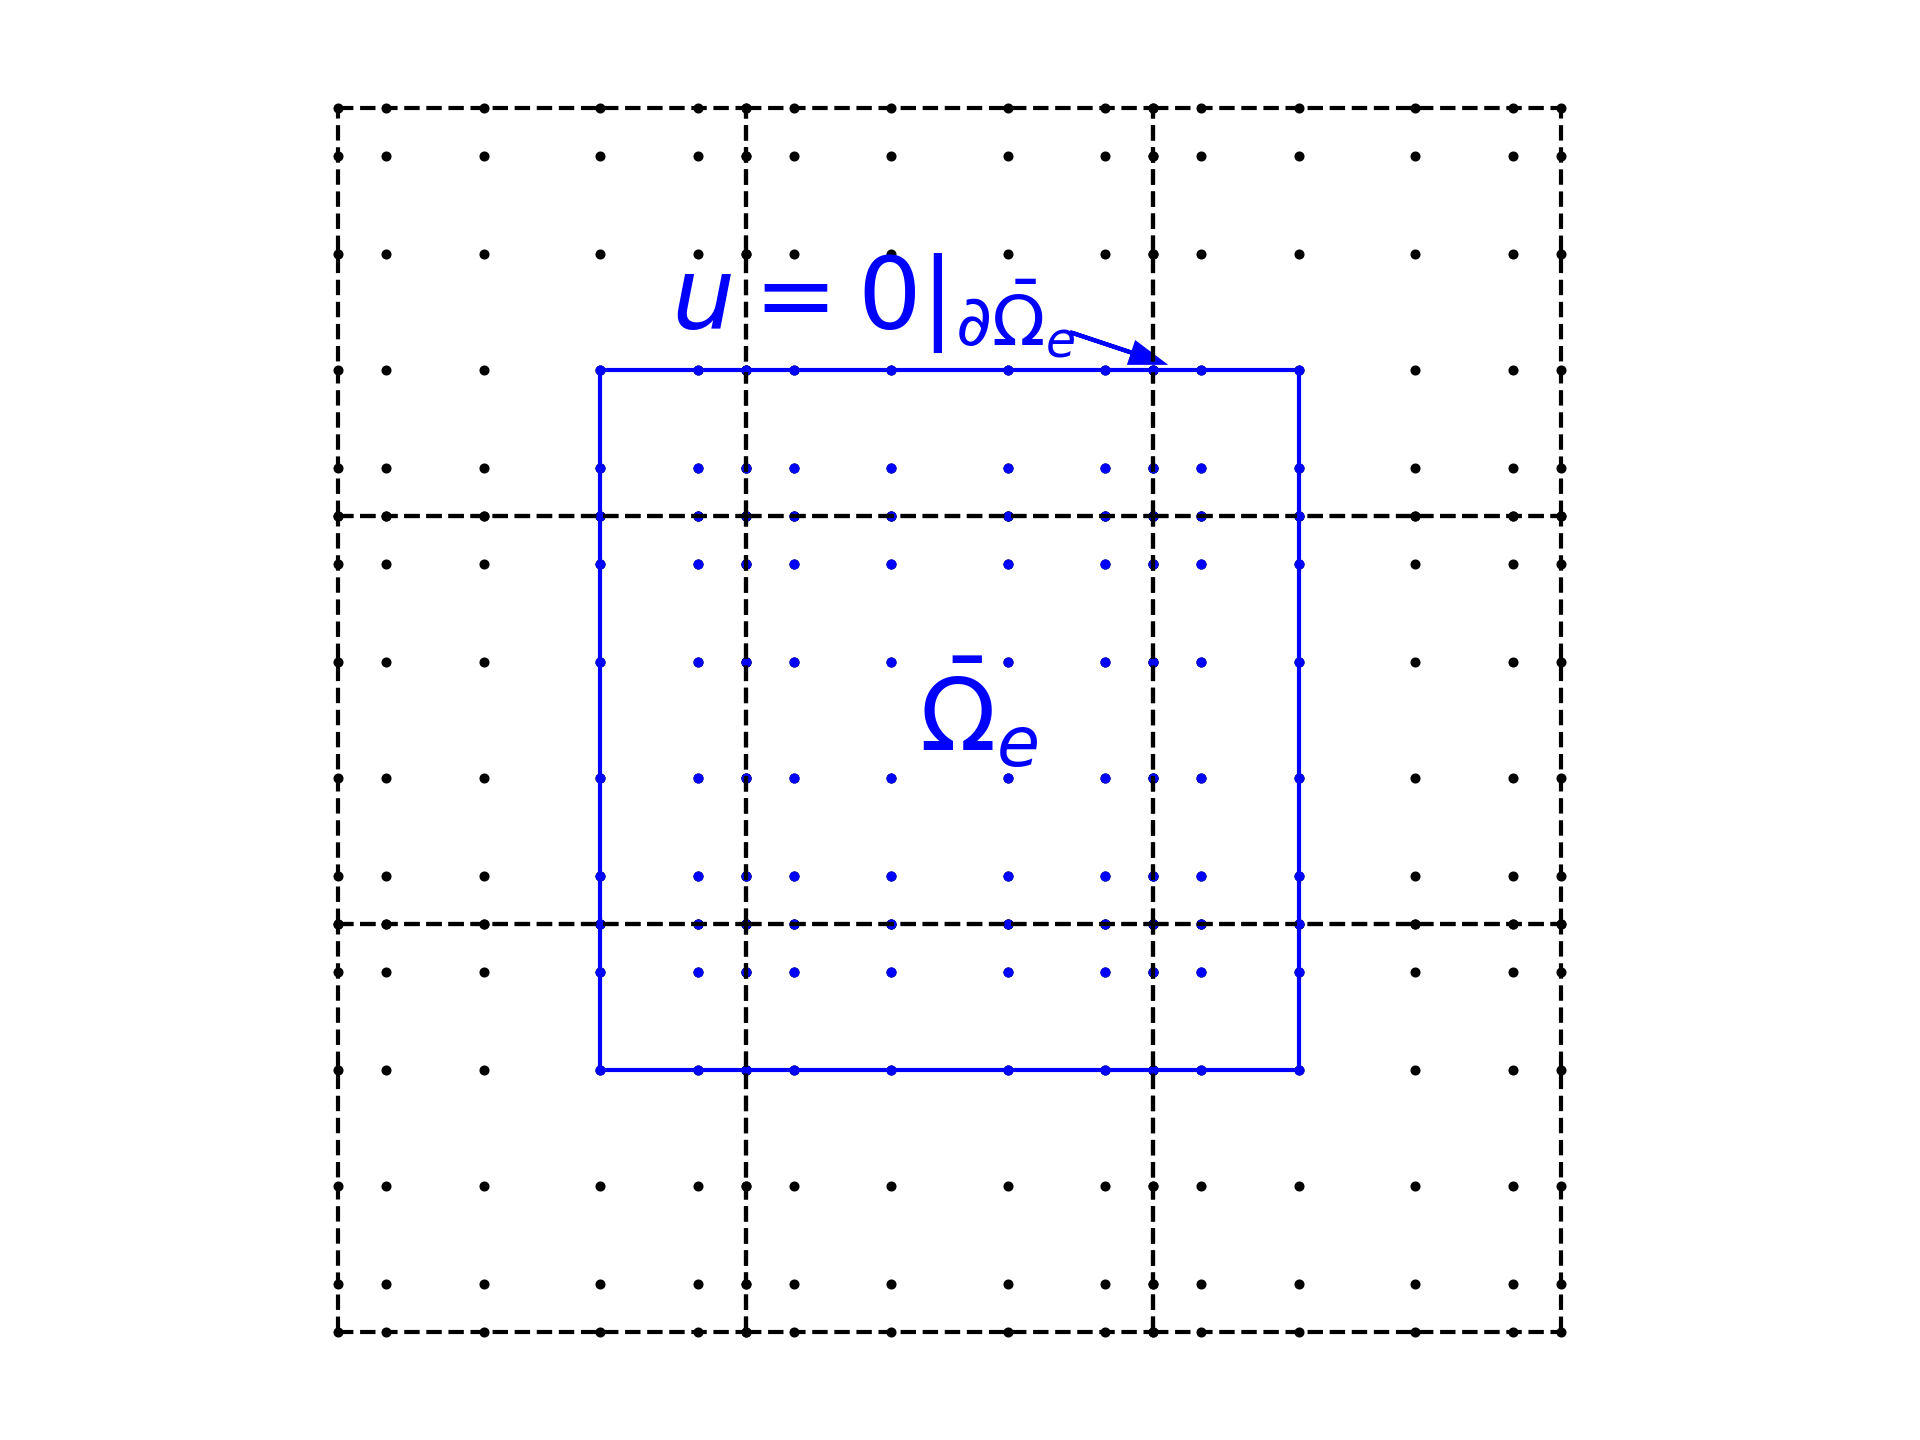
\includegraphics[width=0.5\textwidth]{../figs/overlapping-schwarz-diagram-p=5.png}}
       \put(0.5,0.0){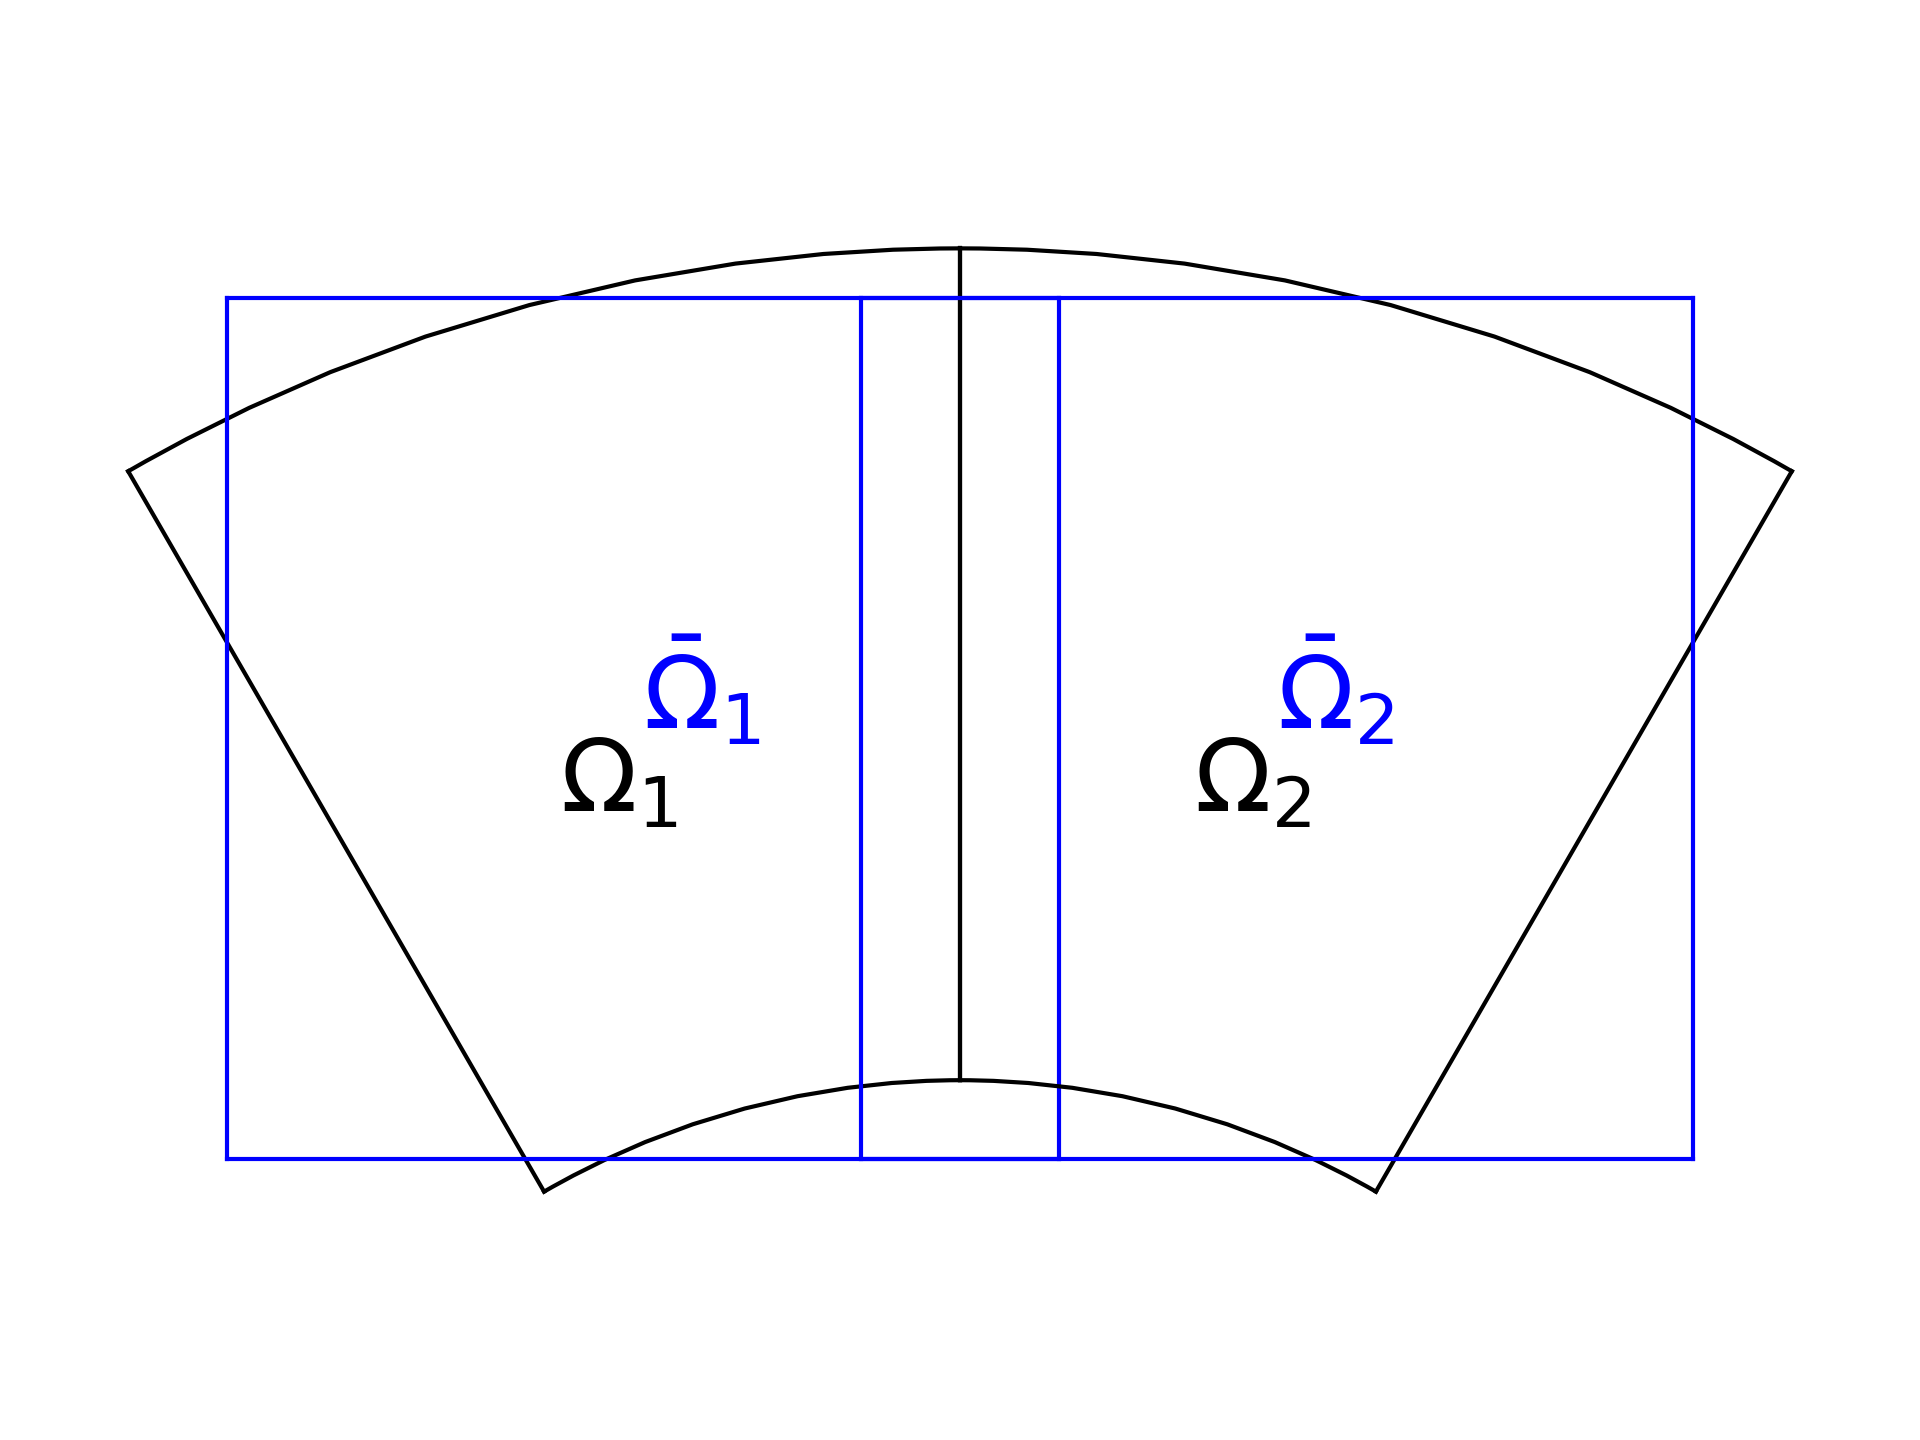
\includegraphics[width=0.5\textwidth]{../figs/schwarz-approximation.png}}
  
       \put(0.0,0.05){\large (a)}
       \put(0.45,0.05){\large (b)}
    \end{picture}
  }
  %\vspace{-0.4cm}
  %\caption{\label{fig:schwarz} Schwarz}
  \end{figure}
  \vspace{-0.65cm}
  \begin{itemize}
    \item $\mathbf M^{-1} := \sum_{e=1}^E \mathbf W_e \mathbf R_e^T \mathbf {\bar A}_e^{-1} \mathbf R_e$, subdomain (a) \footcite{lottes_hybrid_2005,loisel_hybrid_2008}.
    \item How to form $\mathbf {\bar A}_e^{-1}$?
    \begin{itemize}
      \item Galerkin: $\mathbf {\bar A}_e = \mathbf R_e \mathbf A \mathbf R_e^T$, ruins $\mathcal O(p^3)$ storage, $\mathcal O(p^4)$ work per element.
      \item Box-like approximation (b): recover $\mathcal O(p^3)$ storage, $\mathcal O(p^4)$ work per element using fast diagonalization method (FDM).
    \end{itemize}
  \end{itemize}
\end{frame}

%\begin{frame}{FDM}
%  \begin{itemize}
%    \item 3D Poisson-in-a-box:
%      \begin{equation*}\label{eq:tensor-prod-poisson}
%      \mathbf {\bar A} = \mathbf B_z \otimes \mathbf B_y \otimes \mathbf A_x
%               +\mathbf B_z \otimes \mathbf A_y \otimes \mathbf B_x
%               +\mathbf A_z \otimes \mathbf B_y \otimes \mathbf B_x,
%      \end{equation*}
%    \item Directly invert with FDM with $\mathcal O(p^3)$ storage, $\mathcal O(p^4)$ work:
%      \begin{equation*}\label{eq:inverse-tensor-prod-poisson}
%      {\bar A}^{-1} = 
%      (S_z\otimes S_y\otimes S_x) D^{-1} (S_z^T \otimes S_y^T \otimes S_x^T),
%      \end{equation*}
%      where
%      \begin{equation*}
%      D=I\otimes I\otimes \Lambda_x+I\otimes \Lambda_y \otimes I+\Lambda_z \otimes I \otimes I
%      \end{equation*}
%      and each $\mathbf S_*$, $\mathbf \Lambda_*$ are from the generalized eigenvalue problem:
%      \begin{equation*}\label{eq:generalized-eig}
%      \mathbf A_* \mathbf{s}_i = \lambda_i \mathbf B_* \mathbf{s}_i
%      \end{equation*}
%      where $\mathbf B_*$, $\mathbf A_*$ are 1D mass-stiffness matrices.
%  \end{itemize}
%
%\end{frame}